\documentclass[letterpaper]{article}
\usepackage[margin=1in]{geometry}
\usepackage[utf8]{inputenc}
\usepackage{textcomp}
\usepackage{amssymb}
\usepackage{natbib}
\usepackage{graphicx}
\usepackage{gensymb}
\usepackage{amsthm, amsmath, mathtools}
\usepackage[dvipsnames]{xcolor}
\usepackage{enumerate}
\usepackage{mdframed}
\usepackage[most]{tcolorbox}
\usepackage{csquotes}
% https://tex.stackexchange.com/questions/13506/how-to-continue-the-framed-text-box-on-multiple-pages

\tcbuselibrary{theorems}

\newcommand{\R}{\mathbb{R}}
\newcommand{\Z}{\mathbb{Z}}
\newcommand{\N}{\mathbb{N}}
\newcommand{\Q}{\mathbb{Q}}
\newcommand{\C}{\mathbb{C}}
\newcommand{\code}[1]{\texttt{#1}}
\newcommand{\mdiamond}{$\diamondsuit$}
\newcommand{\PowerSet}{\mathcal{P}}
\newcommand{\Mod}[1]{\ (\mathrm{mod}\ #1)}
\DeclareMathOperator{\lcm}{lcm}

%\newtheorem*{theorem}{Theorem}
%\newtheorem*{definition}{Definition}
%\newtheorem*{corollary}{Corollary}
%\newtheorem*{lemma}{Lemma}
\newtheorem*{proposition}{Proposition}


\newtcbtheorem[number within=section]{theorem}{Theorem}
{colback=green!5,colframe=green!35!black,fonttitle=\bfseries}{th}

\newtcbtheorem[number within=section]{definition}{Definition}
{colback=blue!5,colframe=blue!35!black,fonttitle=\bfseries}{def}

\newtcbtheorem[number within=section]{corollary}{Corollary}
{colback=yellow!5,colframe=yellow!35!black,fonttitle=\bfseries}{cor}

\newtcbtheorem[number within=section]{lemma}{Lemma}
{colback=red!5,colframe=red!35!black,fonttitle=\bfseries}{lem}

\newtcbtheorem[number within=section]{example}{Example}
{colback=white!5,colframe=white!35!black,fonttitle=\bfseries}{def}

\newtcbtheorem[number within=section]{note}{Important Note}{
        enhanced,
        sharp corners,
        attach boxed title to top left={
            xshift=-1mm,
            yshift=-5mm,
            yshifttext=-1mm
        },
        top=1.5em,
        colback=white,
        colframe=black,
        fonttitle=\bfseries,
        boxed title style={
            sharp corners,
            size=small,
            colback=red!75!black,
            colframe=red!75!black,
        } 
    }{impnote}
\usepackage[utf8]{inputenc}
\usepackage[english]{babel}
\usepackage{fancyhdr}
\usepackage[hidelinks]{hyperref}

\pagestyle{fancy}
\fancyhf{}
\rhead{Math 170B}
\chead{Wednesday, May 24, 2023}
\lhead{Lecture 23}
\rfoot{\thepage}

\setlength{\parindent}{0pt}

\begin{document}
\section{Quadratic Objectives and Quasi-Newton}
We now want to consider quadratic functions in $m$-dimensions, 
\[a \in \R, \qquad b \in \R^m, \qquad A \in \R^{m \times m} \quad \text{(Symmetric.)}\]
The function of interest is 
\[F(x) = a - b^T x + \frac{1}{2}x^T A x, \qquad x \in \R^m.\]
If $A$ is positive definite, then $F(x)$ is convex and it has a minimum $x^*$. 
\begin{center}
    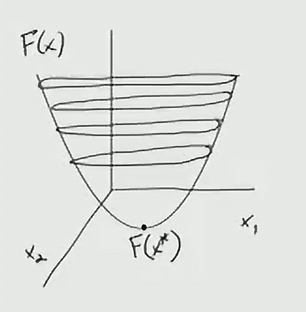
\includegraphics[scale=0.9]{../assets/convex_func.png}
\end{center}
Note that the constant $a$ does not change the location of the minimum. In other words\footnote{$\arg\min_{x \in \R^m} F(x)$ returns the $x$ value corresponding to the smallest $F(x)$.}, \[x^* = \arg \min_{x \in \R^m} F(x) = \arg \min_{x \in \R^m} \left(-b^T x + \frac{1}{2} x^T A x\right).\]
The given derivative is then 
\[F(x) = a - \sum_{i = 1}^{m} b_{i} x_{i} + \frac{1}{2} \underbrace{\sum_{i = 1}^{m} \sum_{j = 1}^{m} x_i A_{ij} x_j}_{\text{Corresponds to } x^T (Ax)}.\]
Its gradient is given by 
\begin{equation*}
    \begin{aligned}
        \frac{\partial F}{\partial x_k} &= \frac{d}{dx_k} \left(a - \sum_{i = 1}^{m} b_{i} x_{i} + \frac{1}{2} \sum_{i = 1}^{m} \sum_{j = 1}^{m} x_i A_{ij} x_j\right) \\ 
            &= -b_{k} + \frac{1}{2} \sum_{j = 1}^{m} A_{kj} x_{j} + \frac{1}{2} \sum_{i = 1}^{m} x_i A_{ik} \\ 
            &= -b_k + 2\left(\frac{1}{2}\right) \sum_{j = 1}^{m} A_{kj} x_j \\ 
            &= -b_k + \left(\frac{1}{2}\right) \sum_{j = 1}^{m} A_{kj} x_j \qquad (1 \leq k \leq m).
    \end{aligned}
\end{equation*}
Note that the above two sums basically produce the same results, but with different indexing. So, we were able to combine them.
\[\nabla F = \begin{bmatrix}
    \frac{\partial F}{\partial x_1} \\ \vdots \\ \frac{\partial F}{\partial x_m}
\end{bmatrix} = \begin{bmatrix}
    -b_1 + \sum_{j = 1}^{m} A_{ij} x_j \\ 
    \vdots \\
    -b_m + \sum_{j = 1}^{m} A_{mj} x_j \\ 
\end{bmatrix} = -b + Ax = g(x).\]
For $1 \leq i \leq m$ and $1 \leq k \leq m$, the Hessian matrix is given by 
\[\frac{\partial^2 F}{\partial x_k \partial x_i} = \frac{d}{dx_i} \left(-b_{k} + \sum_{j = 1}^{m} A_{kj} x_j\right) = A_{ki}.\]
Thus, we can write $\nabla^2 F = A = H(x)$, the entire Hessian matrix.

\subsection{Computing a Minimum}
Suppose the function is convex. If we have $A$ and we can solve for it, then to compute the minimum, we can set the gradient equal to zero: 
\[0 = g(x) = -b + Ax \implies Ax = b \implies A^{-1} b = x.\]
But, in reality, $A$ might be too big, in which case we might consider iteratively solving the minimization problem. In any case, the line-search for quadratic functions can be computed explicitly, by fixing $x^{(k)} \in \R^m$ and $P \in \R^m$, and doing \[\min_{\alpha} F(x^{(k)} + \alpha P).\]
We want to compute the directional derivative, which can be done by solving 
\[\begin{aligned}
    0 &= \frac{d}{d\alpha} F(x^{(k)} + \alpha P) \\
        &= P^T \nabla F(x^{(k)} + \alpha P) \\
        &= P^T \left(A(x^{(k)} + \alpha P) - b\right) \\
        &= P^T (Ax^{(k)} - b) + \alpha P^T AP - P^T (Ax^{(k)} - b) \\
        &= \alpha P^T A P.    
\end{aligned}\]

or just \[\alpha_{k} = \frac{P^T (b - Ax^{(k)})}{P^T a P}.\] $\alpha_k$ is the solution to the line-search problem. The ``residue'' is given by $r^{(k)} = b - Ax^{(k)}$.
\begin{mdframed}
    (Example.) The steepest descent for quadratics is given by 
    \[P^{(k)} = -g(x^{(k)}) = -(Ax^{(k)} - b).\]
    A very brief algorithm is shown below, which takes 
    \begin{itemize}
        \item $x^{(0)}$, the starting point, and 
        \item $M$, the number of iterations,
    \end{itemize}
    as the arguments.
    \begin{algorithm}[H]
        \caption{Steepest Descent}
        \begin{algorithmic}[1]
            \Function{Steepest}{$x^{(0)}, M$}
                \State $k \gets 0$
                \While{$k < M$}
                    \State $x^{(k + 1)} = x^{(k)} + \alpha_{k} P^{(k)}$
                \EndWhile 
            \EndFunction 
        \end{algorithmic}
    \end{algorithm}
\end{mdframed}

\subsection{Quasi-Newton Methods}
An effective class of methods to now consider is the \textbf{Quasi-Newton}. For general nonlinear $F: \R^m \to \R$, we want to only use the gradient function $g(x)$. In other words, we don't need the Hessian matrix here, as computing a Hessian matrix can be quite expensive. So, we can either \emph{approximate} the Hessian matrix\footnote{$H(x_k)$ just means that we're evaluating the Hessian matrix at point $x_k$.}, $H(x_k) \approx B_k$, or approximate the inverse of the Hessian matrix $(H(x_k))^{-1} \approx \hat{H_k}$. These approximations satisfy the secant condition, \[s_k = x_{k + 1} - x_k \in \R^m.\] \[y_j = g_{j + 1} - g_j \in \R^m.\]
We can make use of an algorithm that makes use of this concept. This algorithm, known as the Davidon-Fletcher-Powell Method, takes the following arguments: 
\begin{itemize}
    \item $x_0 \in \R^m$, the starting point; 
    \item $g$, the gradient of $F$; 
    \item $F$, the function itself;
    \item $M$, the maximum number of iterations; and  
    \item $\epsilon$, the tolerance.
\end{itemize}
The algorithm is as follows:
\begin{algorithm}[H]
    \caption{Davidon-Fletcher-Powell Method}
    \begin{algorithmic}[1]
        \Function{Dfp}{$x_0, g, F, M, \epsilon$}
            \State $k \gets 0$
            \State $H_k \gets I$
            \While{$||g(x_k)||_2 > \epsilon$ and $k \leq M$}
                \State $P_k \gets -H_k g(x_k)$
                \State $\alpha_k \gets \min_{\alpha} F(x_k + \alpha P_k)$ \Comment{Line-Search Algorithm}
                \State $s_k \gets \alpha_k P_k$ 
                \State $x_{k + 1} \gets x_k + s_k$ 
                \State $y_k \gets g(x_{k + 1}) - g(x_k)$
                \State $H_k \gets H_k + \frac{s_k s_k^T}{y_k^T s_k} - \frac{H_k y_k y_k^T H_k}{y_k^T H_k y_k}$
                \State $k \gets k + 1$
            \EndWhile 
        \EndFunction
    \end{algorithmic}
\end{algorithm}


\end{document}